\documentclass{article}
\usepackage{fancyhdr}
\usepackage{tikz}
\pagestyle{fancy}
\setlength{\headheight}{35pt}
\lhead{Distributed System I\\Wintersemester2020/21\\Assignment 4}
\chead{}
% bfseries
\rhead{Ciheng Zhang (3472321)\\Chenxi Li(3502796)\\Yaosheng Zheng (3563285)\\Leqi Xu(3556962)}
\cfoot{\thepage}
\renewcommand{\headrulewidth}{0.4pt}

\begin{document}
\begin{titlepage}
    \title{\Huge \textbf{Distributed System I\\Wintersemester2020/21\\Assignment 4} }
    \author{\LARGE \textsl{Ciheng Zhang (3472321) zch3183505@gmail.com}\\\LARGE \textsl{Chenxi Li(3502796) cli216@outlook.com }\\\LARGE \textsl{Leqi Xu(3556962) st176119@stud.uni-stuttgart.de} \\\LARGE \textsl{Yaosheng Zheng (3563285) zhengyaosheng312@icloud.com}\\\LARGE \textsl{Team 19 } \\[200pt]}
    \date{\today}
    \maketitle
    \thispagestyle{empty}
\end{titlepage}
\newpage
\section{Global State}
\subsection*{a)}
$C_1$ is a consistent cut. Because there is no message from future.
\\$C_2$ is not a consistent cut. Because $e_2^4$ need message from future ($e_1^5$)
\subsection*{b)}
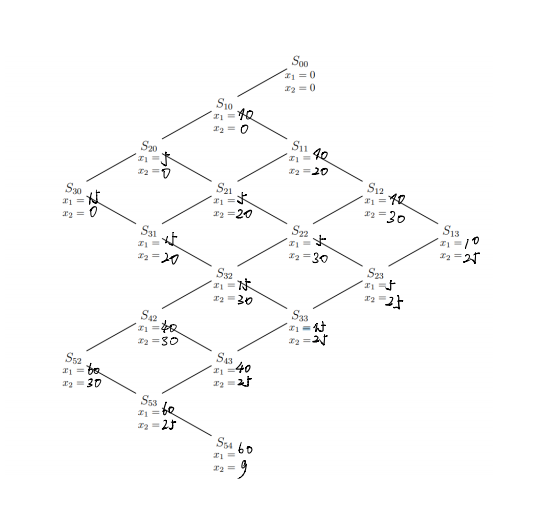
\includegraphics{1_b.png}
\subsection*{c)}
i. $S_{10}$ and $S_{42}$ is true. So its Possibly.
\\ii. $S_{42}$,$S_{43}$,$S_{52}$,$S_{52}$ is true. Every Linearization must pass. So it's definitely.

\section{Transaction Processing}
\subsection*{a)}
4 pairs. \\
1. ${r_1[y],w_2[y]}$\\
2. ${r_1[u],w_3[u]}$\\
3. ${r_2[x],w_3[x]}$\\
4. ${w_2[y],r_3[y]}$
\subsection*{b)}
\begin{tikzpicture}[scale=1.5]
    \node at (0,0) {T3};
    \node at (3,0) {T1};
    \node at (6,0) {T2};

    \draw[->](0.5,0)--(2.5,0);
    \draw[->](3.5,0)--(5.5,0);
    \draw[->](6,0.2)..controls(4.5,1) and(1.5,1)..(0,0.2);
    
\end{tikzpicture}
\\
\begin{tikzpicture}[scale=1.5]
    \node at (0,0) {T3};
    \node at (3,0) {T1};
    \node at (6,0) {T2};

    \draw[->](0.5,0)--(2.5,0);
    \draw[->](3.5,0)--(5.5,0);
    \draw[->](0,0.2)..controls(4.5,1) and (1.5,1)..(6,0.2);
    \draw[->](6,-0.2)..controls(5,-1) and (4,-1)..(3,-0.2);
\end{tikzpicture}
\\Both Serialization graphs have cycle. So both are not serialisable history.

\section{Two-Phase Locking}
From the last question. H3 is not serialisable history. So only H1 and H2 can be generated by 2-phase-Locking.
\\Because:
$r_3[w]<w_2[w],r_2[y]<w_3[y]$
\\
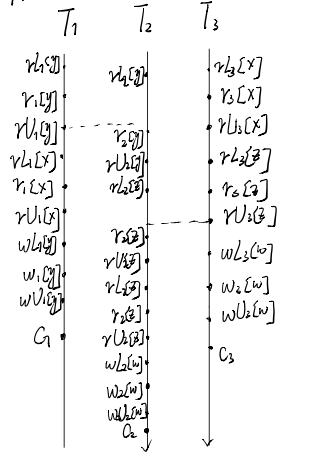
\includegraphics{3H1.png}
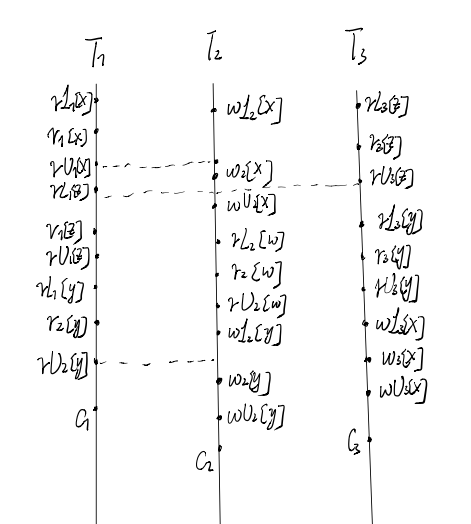
\includegraphics{3h2.png}
\end{document}
